\documentclass{article}
\usepackage[utf8]{inputenc}
\usepackage{caption}
\usepackage[margin=1in]{geometry}
\usepackage{graphicx}
\usepackage{pdfpages}
\usepackage{float}
\pdfminorversion=7

\begin{document}
\begin{titlepage}


\centering
\vspace*{2cm}
{\Huge User Interface Design Document\par}
\vspace{.25cm}
{\LARGE Course Evaluation System\par}
\vspace{1cm}
{\Large Team EVAL\par}
\vspace{.2cm}
{\Large Jovon Craig, Sam Elliott, Robert Judkins, and Stanley Small\par}
\vspace{1cm}
{\Large Client: Dr. Harlan Onsrud\par}
\vspace{1cm}
{\Large November 30, 2018\par}
\vspace{11cm}

University of Maine - Fall of 2018 - COS 397

Instructor: Professor Terry Yoo

\end{titlepage}

\newpage

\begin{center}
{
\includegraphics[scale=.2]{images/team_logo.png}} \\ 	\bigskip
{\LARGE Course Evaluation System } \\ \medskip
{\large User Interface Design Document } \\ \medskip
\end{center}

\tableofcontents

\newpage

\section{Introduction}
 

\subsection{Purpose of This Document}

This user interface design document is an overview of the graphics and layouts shown to the users of our course evaluation system. The first section, the user interface standards, describes the general features of the graphics, such as layouts and components, that are common to all screens in the interface. The second section, the user interface walkthrough, includes a ``navigation diagram'' of the order in which the screens are shown, and complete wireframes of each screen. The docuement's third section gives the data items typically entered in the user interface and how they are formatted.

This document is intended for the development team, the product client, Dr. Harlan Onsrud, and potential users of the system. Team EVAL needs this document to properly implement the user interface in code. Dr. Onsrud also needs it to verify that the program's appearance looks appropriate for universities and to suggest revisions to the UI. Lastly, the document helps the software's users, serving as a guide on how to use the software.


\subsection{References}

Craig, J., Elliott, S., Judkins, R., \& Small, S. 29 October 2018. \textit{System Requirements Specification.}
\vspace{3mm}\newline
Craig, J., Elliott, S., Judkins, R., \& Small, S. 16 November 2018. \textit{System Design Document.}
\vspace{3mm}\newline
Onsrud, H. ``Example Question Selection Form.'' See Appendix D.
\vspace{3mm}\newline
Onsrud, H. ''Report for Professor: Roy Turner'' See Appendix E.

\section{User Interface Standards}

The interface of the course evaluation system is standardized in that several features are present in multiple screens. Figure 1, shown on the next page, is the overall screen layout of our course evaluation system. It shows the general areas and components of the screens in the user interface. Not all screens follow this exact overall layout.

\newpage

\begin{center}
\captionof{figure}{Overall layout of a screen in the UI}
\vspace{3mm}
{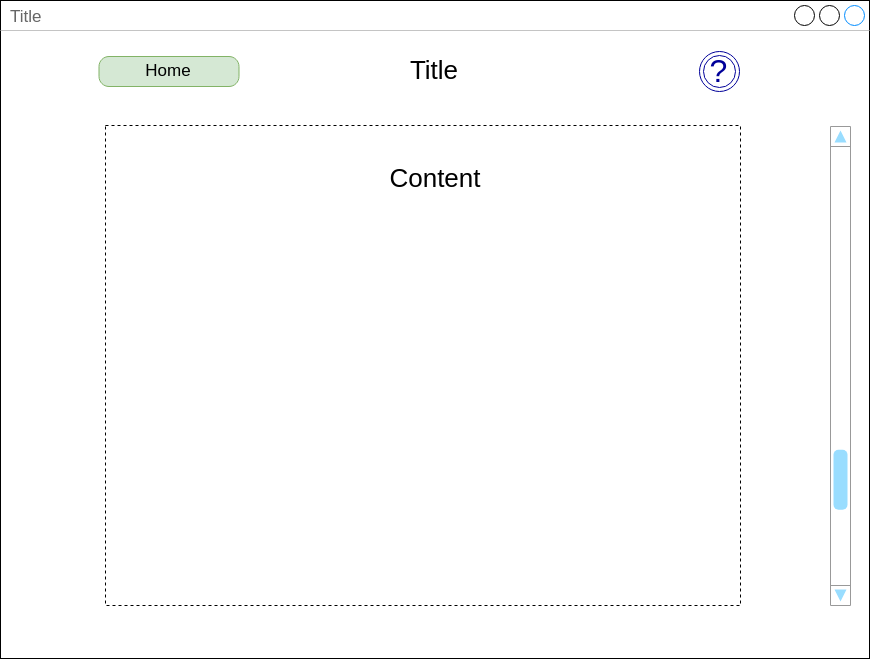
\includegraphics[scale=0.5]{images/overall_layout.png}}
\vspace{2mm}
\end{center}

For ease of use, the team made the designs simple for each of the screens. On the top-left corner, there is a button to return the user to the home page (or the log-in screen if the user is at the home page). To the right is the page title, which summarizes the purpose of the screen. The top-right corner includes the help button, which directs the user to the help screen. The ``content'' is located below the top elements, containing instructions, data entry fields, and the like.  For sections that may be complicated a help pop up will appear when mousing over the question mark icon. Most screens also have a scroll bar on the right side if the information on a page cannot all fit in the web browser.

\section{User Interface Walkthrough}

This section goes into more detail about the screens in the user interface and how an administrator or instructor navigates through them. Figure 2 on the next page is the navigation diagram, which shows the paths that a user can take through the system's interface. The diagram also includes the names for all the screens in the UI.

\newpage

\begin{center}
\captionof{figure}{Navigation diagram of the user interface}
\vspace{3mm}
{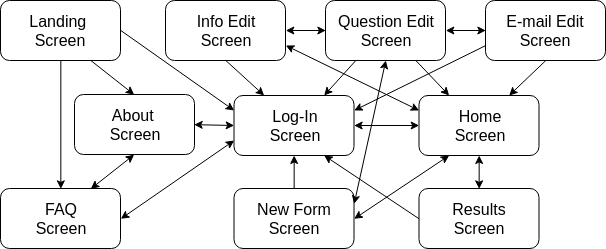
\includegraphics[scale=0.6]{images/navigation_diagram.png}}
\vspace{2mm}
\end{center}

The first screen that the user sees upon starting up the system is the \textbf{Landing Screen}. The user can switch between that and both the \textbf{FAQ Screen} and  \textbf{Log-In Screen}. After entering a correct username and password on the log-in screen, the \textbf{Home Screen} appears. The user can then call up the \textbf{Info Edit Screen}, \textbf{New Form Screen}, or \textbf{Results Screen} from the home page. To edit an evaluation form, a user must go to the info edit screen, then the \textbf{Question Edit Screen}, then the \textbf{E-mail Edit Screen}. The log-in screen and home screen can be accessed from any other screen except the about and FAQ screens.

The next set of figures, Figures 3 to 11, consist of the wireframes for each screen in the evaluation system. These diagrams communicate the areas, menus, and buttons that are unique to a certain screen and what they do.

\newpage
\newgeometry{left=1in, right=1in, top=2cm, bottom=2cm}

\begin{center}
\begin{figure}[H]
    \centering
    \caption{Landing screen}
    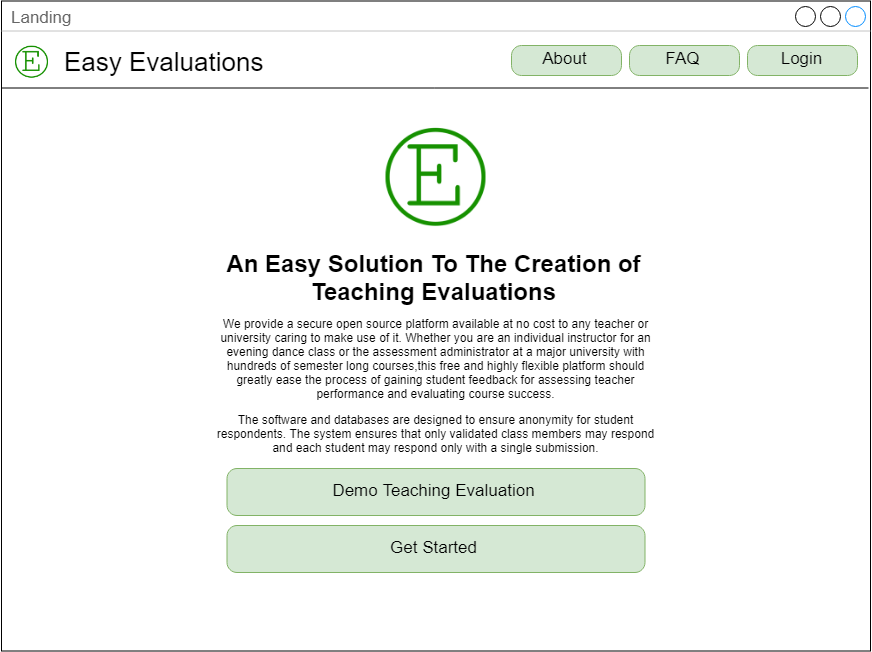
\includegraphics[scale=.35]{images/landing_screen.png}
\end{figure}
\end{center}

This is the first screen a user would see when they enter the website. A user could click on the `Demo Teaching Evaluation' button that would link to an informative video. Clicking `Get Started' would lead them to an account creation screen. Alternatively they could click `About', `FAQ', or `Sign In' to enter the corresponding screens.

\begin{center}
\begin{figure}[H]
    \centering
    \caption{Log-in screen}
    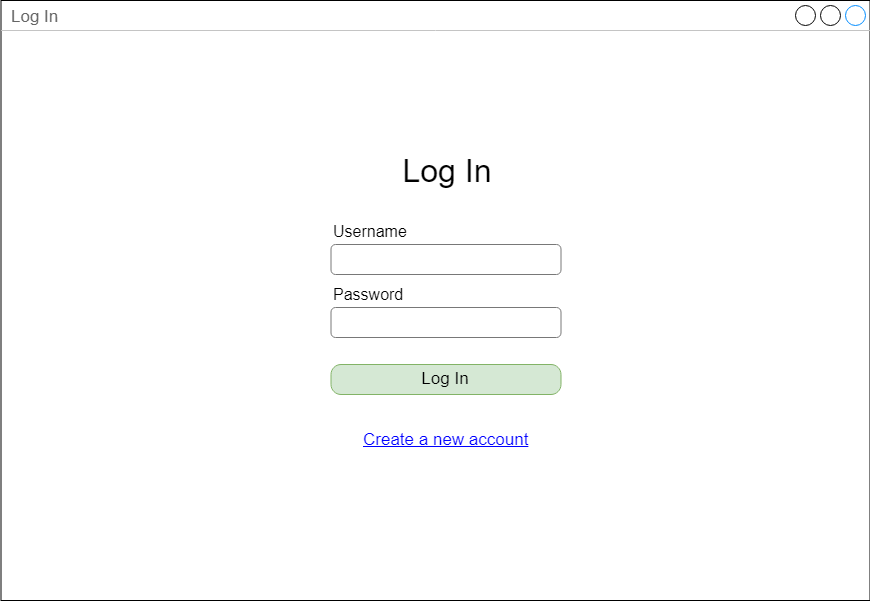
\includegraphics[scale=.35]{images/login_screen.png}
\end{figure}
\end{center}

A user would enter a valid username and password and login. Clicking `Log In' advances the user to the Selection Screen.  The about, FAQ, and Sign In buttons would take you to their respective pages.

\begin{center}
\begin{figure}[H]
    \centering
    \caption{FAQ Screen}
    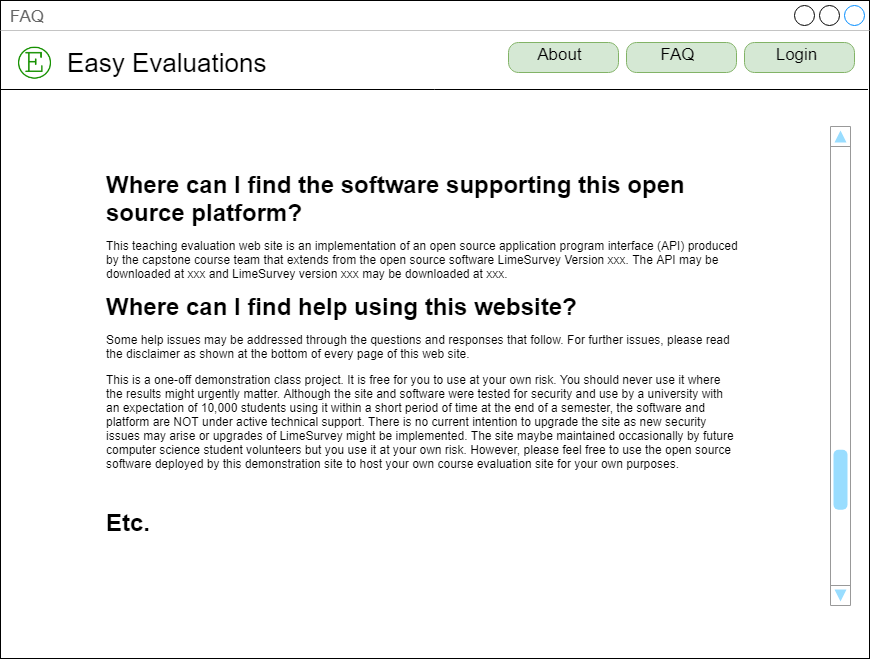
\includegraphics[scale=.35]{images/faq_screen.png}
\end{figure}
\end{center}

This screen details frequently asked questions a user may have and their corresponding answers. The about, FAQ, and Sign In buttons would take you to their respective pages.

\begin{center}
\begin{figure}[H]
    \centering
    \caption{About screen}
    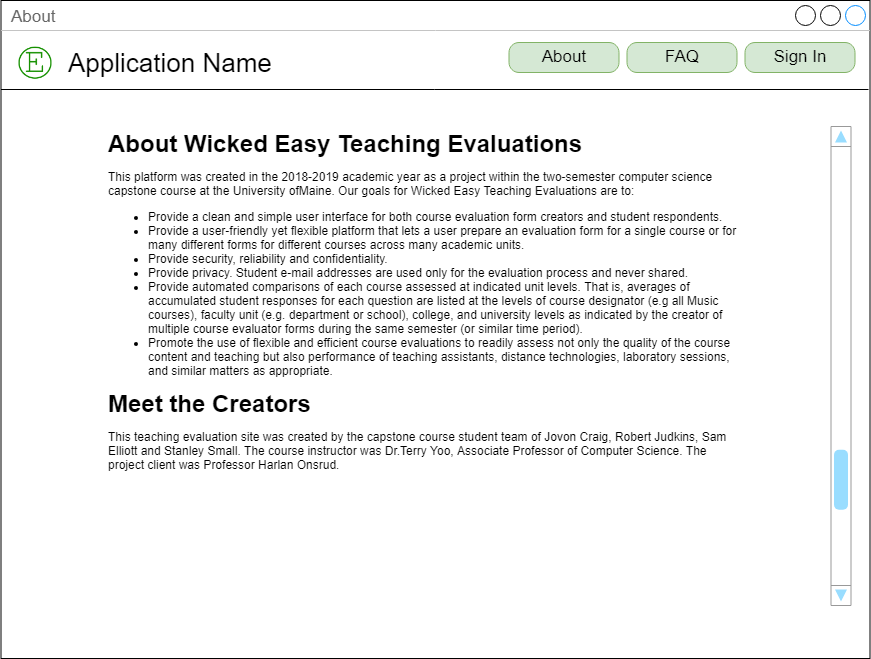
\includegraphics[scale=.35]{images/about_screen.png}
\end{figure}
\end{center}

This screen gives details about the product and its purpose. It also credits the creators as well as the client for whom the product was made.  The about, FAQ, and Sign In buttons would take you to their respective pages.

\begin{center}
\begin{figure}[H]
    \centering
    \caption{Home screen}
    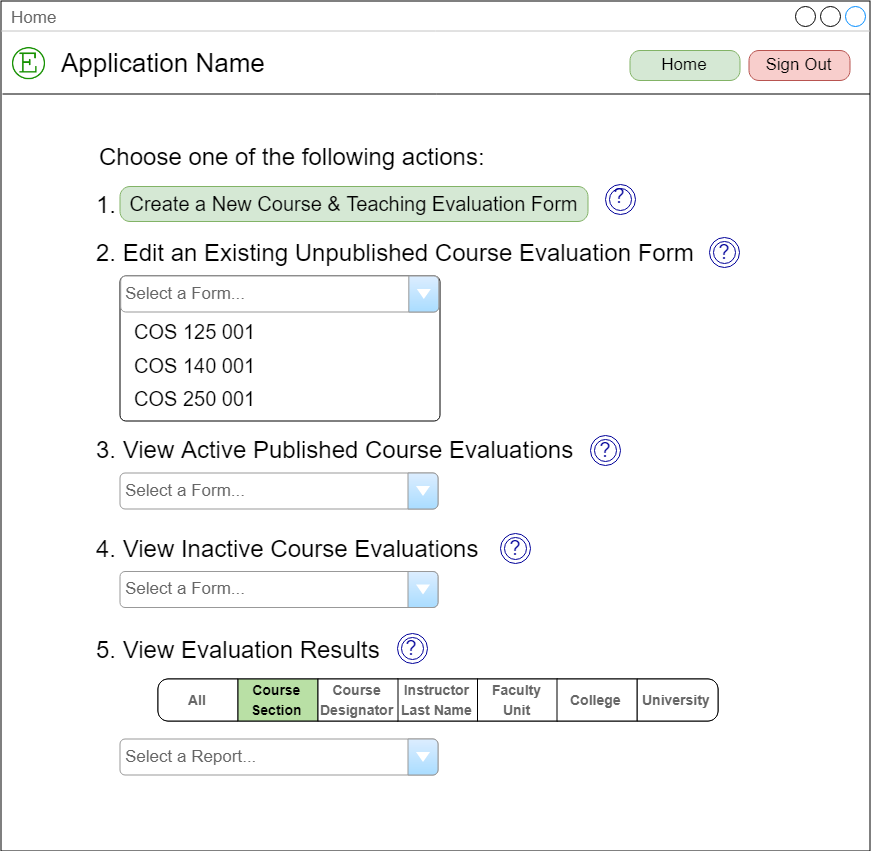
\includegraphics[scale=.25]{images/home_screen.png}
\end{figure}
\end{center}

This is the main screen a user would see after they login. They can choose to create a new evaluation (1) which will redirect them to the new form screen. Select a course which they had published (2) which will redirect to the edit info screen where they view but not edit information.  They can select a course that has already been completed (3) which will redirect them to the edit screen to view but not edit information.  They can select a category to view results by, then choose a section of that category with the drop down menu (5) which will redirect them to the results page.

\begin{center}
\begin{figure}[H]
    \centering
    \caption{New form screen}
    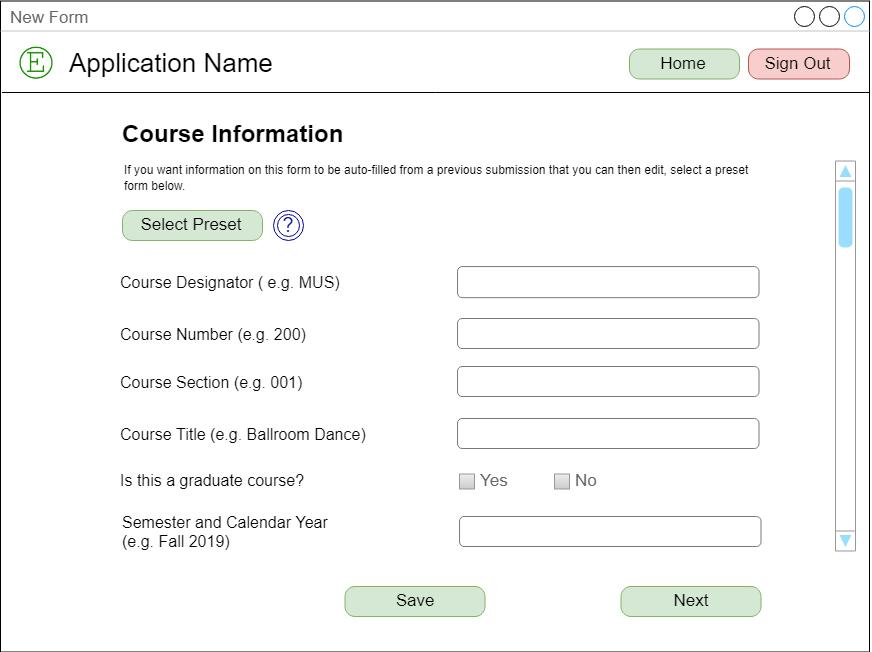
\includegraphics[scale=.35]{images/create_screen.png}
\end{figure}
\end{center}

This is the page a user would see if they decided to create a new evaluation. This page asks the user to fill out the general information of the course they're creating the evaluation for. Alternatively they can select a previously created preset rather than starting from scratch.  See Appendix D for a full example.

\begin{center}
\begin{figure}[H]
    \centering
    \caption{Edit Info screen}
    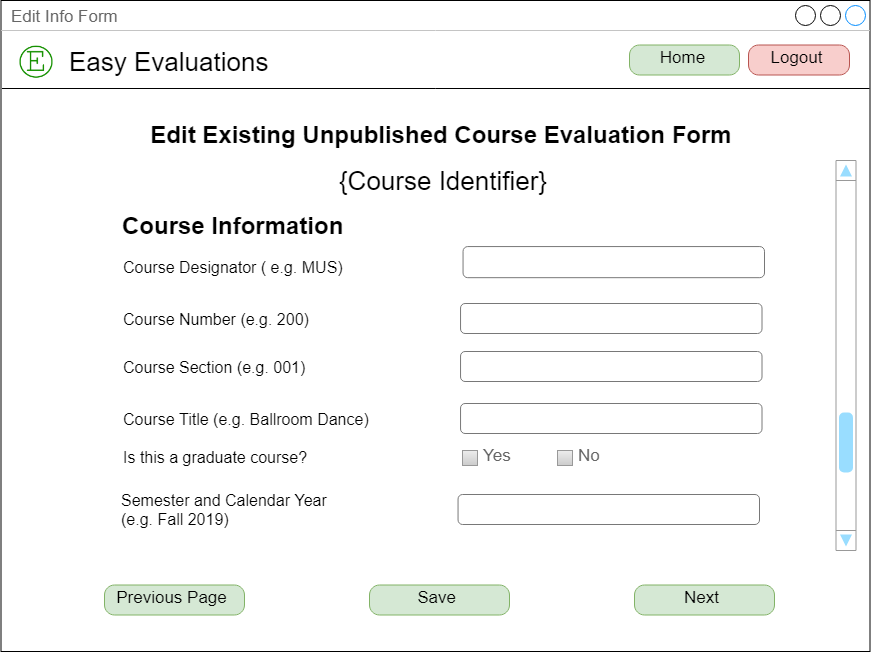
\includegraphics[scale=.30]{images/edit_info_screen.png}
\end{figure}
\end{center}

Much similar to the new form screen, a user would will be redirected to this screen when they choose to edit a evaluation they've created. It allows them to view and edit the information of an existing evaluation.  The previous button will redirect the user to the home page, the next button will redirect them to the question edit screen and the save button will save the entered information. See Appendix D for a full example.

\begin{center}
\begin{figure}[H]
    \centering
    \caption{Question edit screen}
    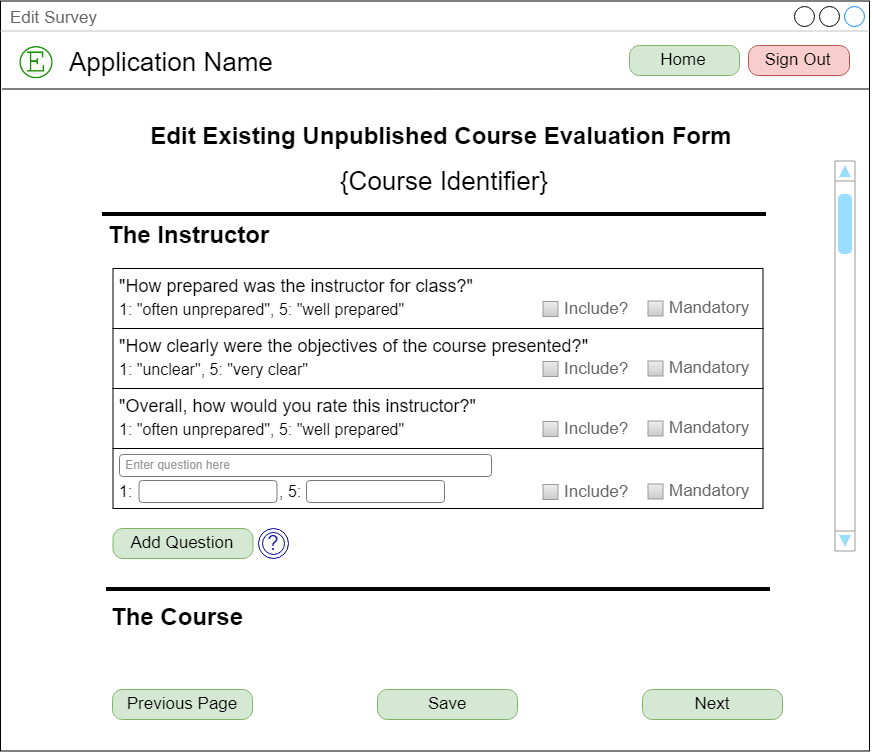
\includegraphics[scale=.30]{images/questions_screen.png}
\end{figure}
\end{center}

This is the second page a user would see when they are creating a course evaluation, they will be redirected here when they press the next button from the create form page or edit info page.  The previous button will redirect them to the question edit screen, the next button will redirect them to the E-mail edit screen and the save button will save the entered data. It lists several generic questions that may be asked in a evaluation and asks if the instructor would like to include it and whether or not it should be mandatory. They can also add custom questions at each section.  See Appendix D for a full example.

\begin{center}
\begin{figure}[H]
    \centering
    \caption{E-mail edit screen}
    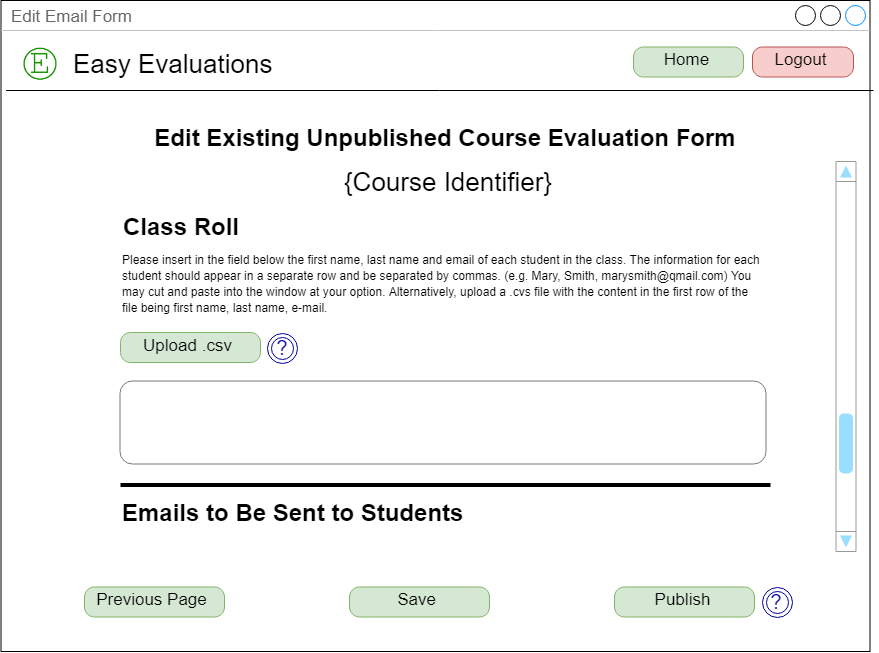
\includegraphics[scale=.30]{images/emails_screen.png}
\end{figure}
\end{center}

This is the final page a user would see when creating a new course evaluation. They will be redirected here when the next button is pressed on the Question Edit Screen. It asks the instructor to include a list of students taking the course, to review a generic email that would be sent to students, and to review a reminder email that could be sent after a certain period of time. See Appendix D for a full example.

\begin{center}
\begin{figure}[H]
    \centering
    \caption{Results screen}
    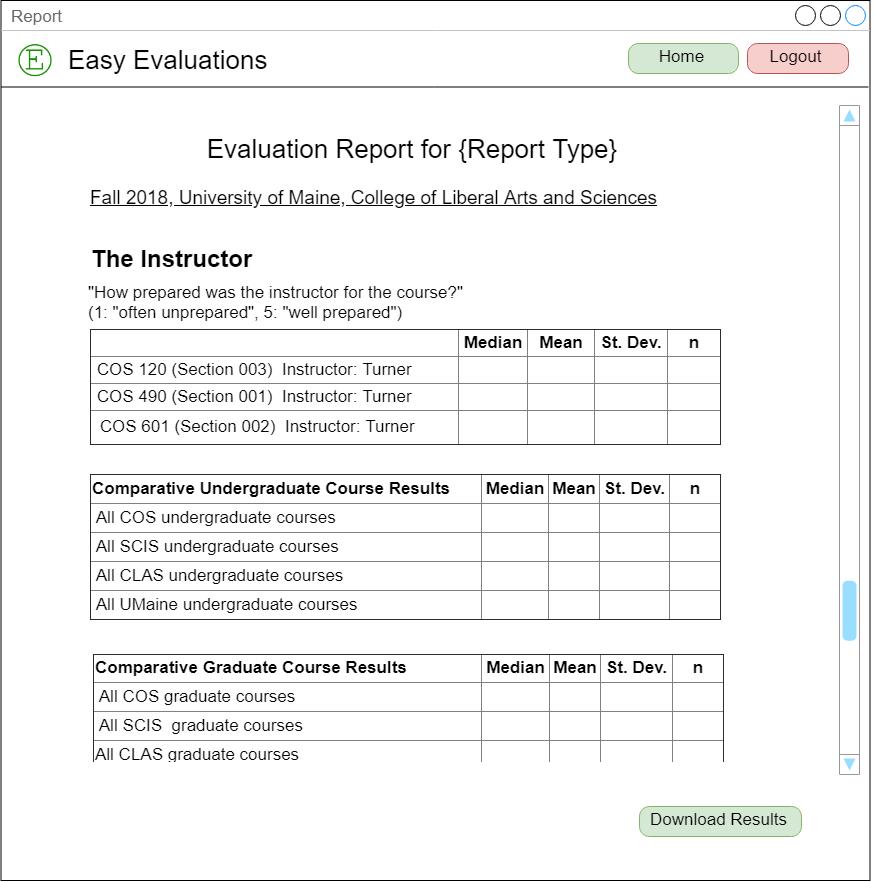
\includegraphics[scale=.25]{images/report_screen.png}
\end{figure}
\end{center}

This page is where a user would view results of their evaluations based on the category selected when being redirected here from the home screen.  The responses organized by each question in the evaluation and displays different tables for undergraduate courses and graduate courses. It includes the median, mean, standard deviation, and number of answers for each question along with statistics on the question for categories the classes are included in. The results can also be downloaded and exported as a .csv file by clicking the download results button. See Appendix D for a full example.

\section{Data Validation}

Table 1 on the next page lists the data items in the user interface of the evaluation system. A data item is an input that a user enters into the system and has a specified format. As shown on the next page, many items are for editing an evaluation evaluation form.

\newpage
\newgeometry{left=1cm, right=1cm, top=1in, bottom=1in}
\begin{center}
\captionof{table}{Data item specification}
\scalebox{.90}{
\begin{tabular}{|p{4.4cm}|p{2.2cm}|p{1.5cm}|p{4cm}|p{3cm}|} 
\hline
\textbf{Label} & \textbf{Screen(s)} & \textbf{Data Type} & \textbf{Format} & \textbf{Limit(s)} \\
\hline
Username & Log in & String & username@gmail.com & N/A \\ 
\hline
Password &New/Edit form & String & N/A & N/A \\ 
\hline
Course designator & New/Edit form & String & N/A & 50 characters \\ 
\hline
Course number &New/Edit form & String & N/A & 50 characters\\ 
\hline
Course section &New/Edit form & String & N/A & 50 characters\\ 
\hline
Course title & New/Edit form & String & N/A & 50 characters\\ 
\hline
Graduate Course & New/Edit form & Boolean & N/A & 50 characters\\ 
\hline
Semester and year &New/Edit form & String & N/A & 50 characters\\ 
\hline
Faculty unit & New/Edit form & String & N/A & 50 characters\\ 
\hline
Department & New/Edit form & String & N/A & 50 characters\\ 
\hline
University &New/Edit form & String & N/A & 50 characters\\ 
\hline
Instructor first name &New/Edit form & String & N/A & 50 characters \\ 
\hline
Instructor last name & New/Edit form & String & N/A & 50 characters\\ 
\hline
Instructor e-mail & New/Edit form & String & N/A & 50 characters\\ 
\hline
Instructor phone & New/Edit form & String & N/A & 50 characters\\ 
\hline
Course evaluation administrator & New/Edit form & String & N/A & 50 characters\\ 
\hline
Evaluation administrator e-mail & New/Edit form & String & N/A & 50 characters\\ 
\hline
Starting assessment date & String & New/Edit form & mm/dd/yy & 50 characters\\ 
\hline
Mailing time & New/Edit form & String & hr:min:sec & 50 characters\\ 
\hline
Closing assessment date & New/Edit form & String & N/A & 50 characters\\ 
\hline
Added question & Question edit & Strings & N/A & 150 characters\\ 
\hline
1 score label & Question edit & String & N/A & 50 characters\\
\hline
5 score label & Question edit & String & N/A & 50 characters\\
\hline
``Include?'' checkboxes & Question edit & Boolean & N/A & N/A \\ 
\hline
``Mandatory'' checkboxes & Question edit & Boolean & N/A & N/A \\ 
\hline
Class roll & E-mail edit & String & Comma separated: \newline first,last,email & N/A \\ 
\hline
Initial e-mail to students & E-mail edit & String & N/A & N/A \\ 
\hline
Reminder e-mail & E-mail edit & String & N/A & N/A\\ 
\hline
Final confirmation e-mail & E-mail edit & String & N/A & N/A\\ 
\hline
\end{tabular}
}
\end{center}

\appendix
\newgeometry{left=1in, right=1in, top=1in, bottom=1in}

\newpage
\section{Agreement Between Customer and Contractor}
This page shows that all members of Team EVAL and the client, Harlan Onsrud, have agreed on all the information in the user interface design document. By signing this document, Team EVAL and Dr. Onsrud approve all of the designs for each screen in the interface, as well as how to navigate the interface.

The team will follow a process in the case that the design document is changed after we sign it. First, the team will write a rough draft of the changes to be made to the document. Second, all team members and Harlan Onsrud will sign the document agreeing to the changes. Finally, the team will make the changes to the final copy of the document.

\vspace{.7in}
\noindent
\begin{tabular}{ p{5cm} p{5cm} p{5cm} } 
\textbf{\textit{Name}} & \textbf{\textit{Signature}} & \textbf{\textit{Date}} \\[.5cm]
\textbf{Jovon Craig} & $\rule{5cm}{.1mm}$ & $\rule{5cm}{.1mm}$\\[.5cm]
\textbf{Sam Elliott} & $\rule{5cm}{.1mm}$ & $\rule{5cm}{.1mm}$\\[.5cm]
\textbf{Robert Judkins} & $\rule{5cm}{.1mm}$ & $\rule{5cm}{.1mm}$\\[.5cm]
\textbf{Stanley Small} & $\rule{5cm}{.1mm}$ & $\rule{5cm}{.1mm}$\\[.5cm]
\textbf{Harlan Onsrud} & $\rule{5cm}{.1mm}$ & $\rule{5cm}{.1mm}$\\[.5cm]
Customer Comments: & \multicolumn{2}{ l }{ $\rule{10.45cm}{.1mm}$ }\\[.5cm]
\multicolumn{3}{ l }{ $\rule{15.9cm}{.1mm}$ }\\[.5cm]
\end{tabular}

\newpage
\section{Team Review Sign-off}

This page shows that all members of Team EVAL have reviewed the user interface design document and agreed on its content. By signing this document, the team members agree that all information about the evaluation system's UI is accurate, and that there is nothing in the document that is a source of contention.

\vspace{.7in}
\noindent
\begin{tabular}{ p{5cm} p{5cm} p{5cm} } 
\textbf{\textit{Name}} & \textbf{\textit{Signature}} & \textbf{\textit{Date}} \\[.5cm]
\textbf{Jovon Craig} & $\rule{5cm}{.1mm}$ & $\rule{5cm}{.1mm}$\\[.5cm]
Comments: & \multicolumn{2}{ l }{ $\rule{10.45cm}{.1mm}$ }\\[.5cm]
\multicolumn{3}{ l }{ $\rule{15.9cm}{.1mm}$ }\\[.5cm]
\textbf{Sam Elliott} & $\rule{5cm}{.1mm}$ & $\rule{5cm}{.1mm}$\\[.5cm]
Comments: & \multicolumn{2}{ l }{ $\rule{10.45cm}{.1mm}$ }\\[.5cm]
\multicolumn{3}{ l }{ $\rule{15.9cm}{.1mm}$ }\\[.5cm]
\textbf{Robert Judkins} & $\rule{5cm}{.1mm}$ & $\rule{5cm}{.1mm}$\\[.5cm]
Comments: & \multicolumn{2}{ l }{ $\rule{10.45cm}{.1mm}$ }\\[.5cm]
\multicolumn{3}{ l }{ $\rule{15.9cm}{.1mm}$ }\\[.5cm]
\textbf{Stanley Small} & $\rule{5cm}{.1mm}$ & $\rule{5cm}{.1mm}$\\[.5cm]
Comments: & \multicolumn{2}{ l }{ $\rule{10.45cm}{.1mm}$ }\\[.5cm]
\multicolumn{3}{ l }{ $\rule{15.9cm}{.1mm}$ }\\[.5cm]
\end{tabular}


\newpage
\section{Document Contributions}

Stanley Small contributed to the discussion of the UI design. Stan contributed approximately 5 percent of the document.

Jovon Craig wrote the purpose of the document, the user interface standards section, the description of the UI navigation, the first three columns of the data item table, and Appendix C. He created the overall layout diagram, navigation diagram, and many of the individual screen layouts. Jovon contributed about 35 percent of the document.

Sam Elliott revised all of the individual screen layouts and added several new screens. He also wrote the last two columns in the data item table. Sam contributed about 40 percent of the document.

Robert Judkins converted the UIDD template to the LaTeX format and placed it in our document. He wrote the descriptions under each wireframe picture of the UI. He also added the references and appendices A, B, and D. Robert contributed about 20 percent of the document.

\newpage

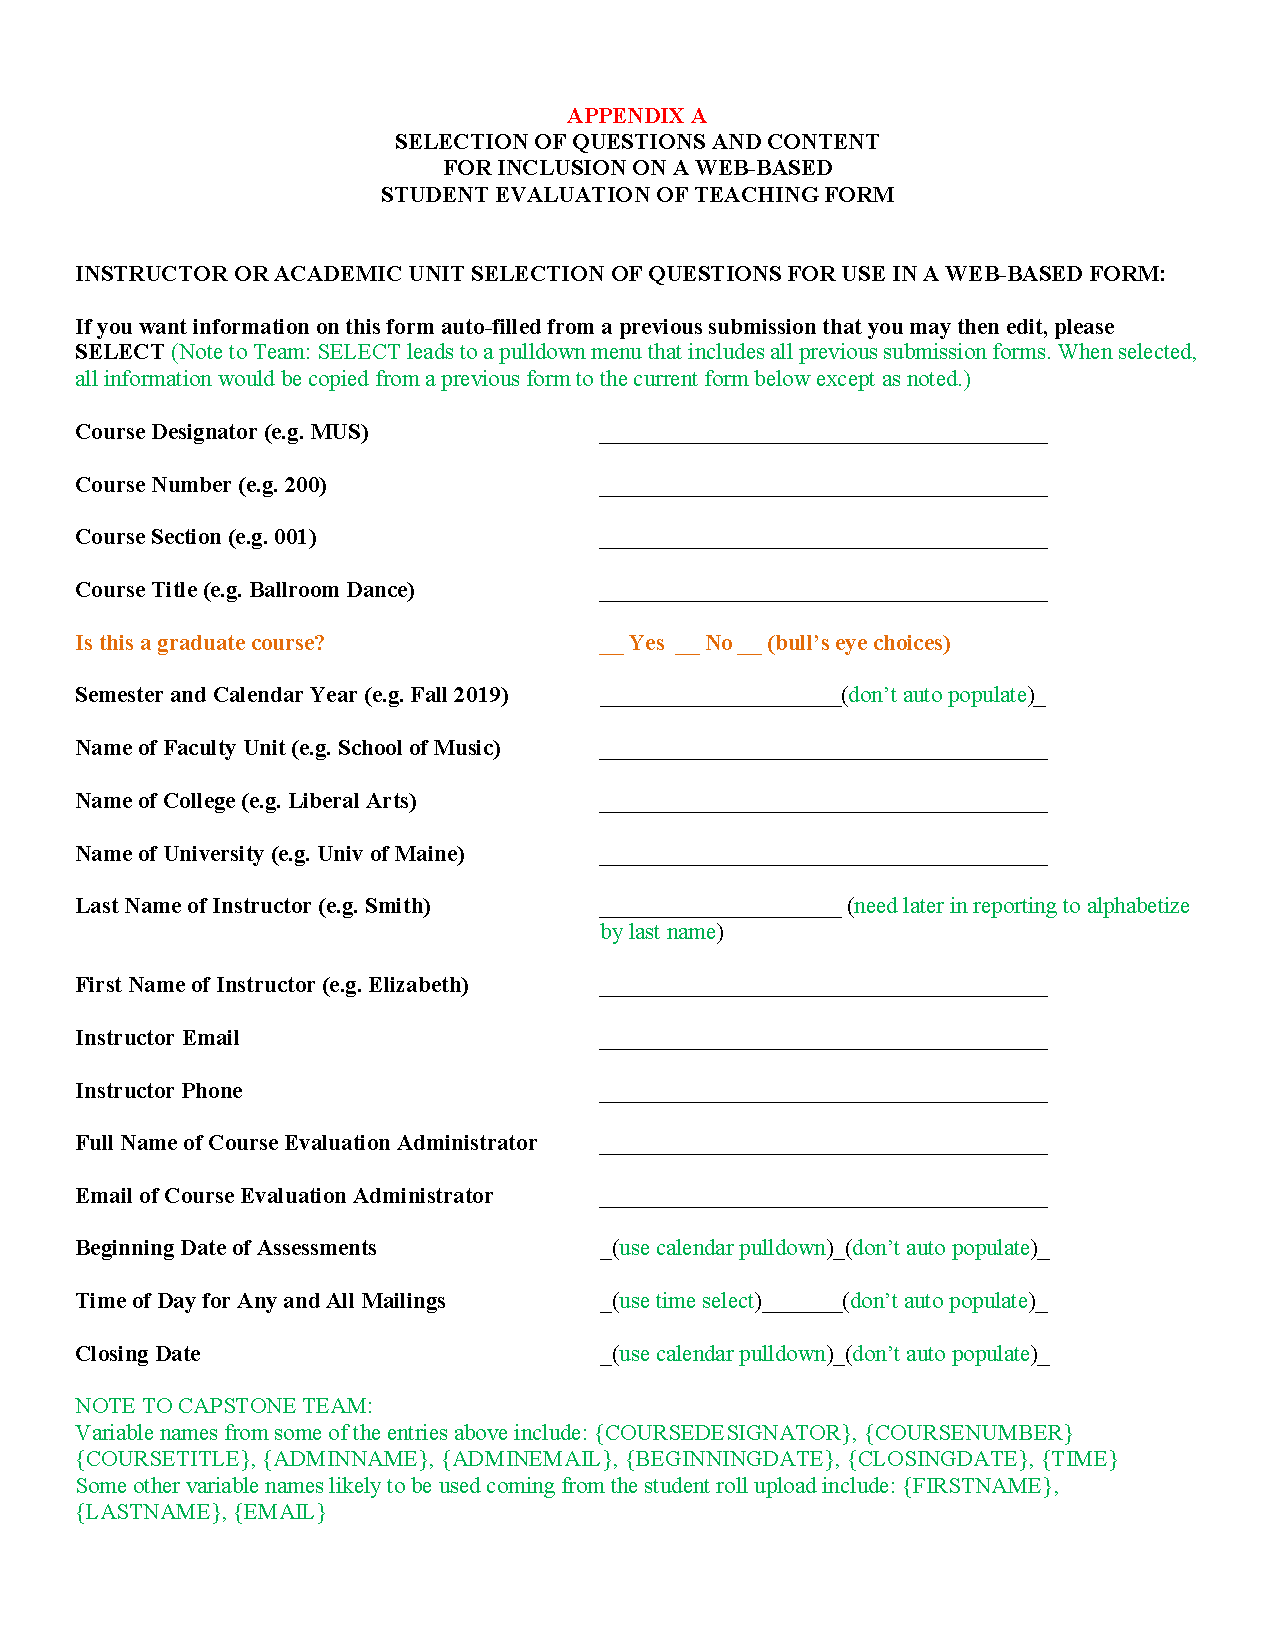
\includepdf[scale=0.85,pages=1,pagecommand=\section{Example Question Selection Form}]{images/question_appendix.pdf}
\includepdf[scale=0.85,pages=2-]{images/question_appendix.pdf}

\newpage

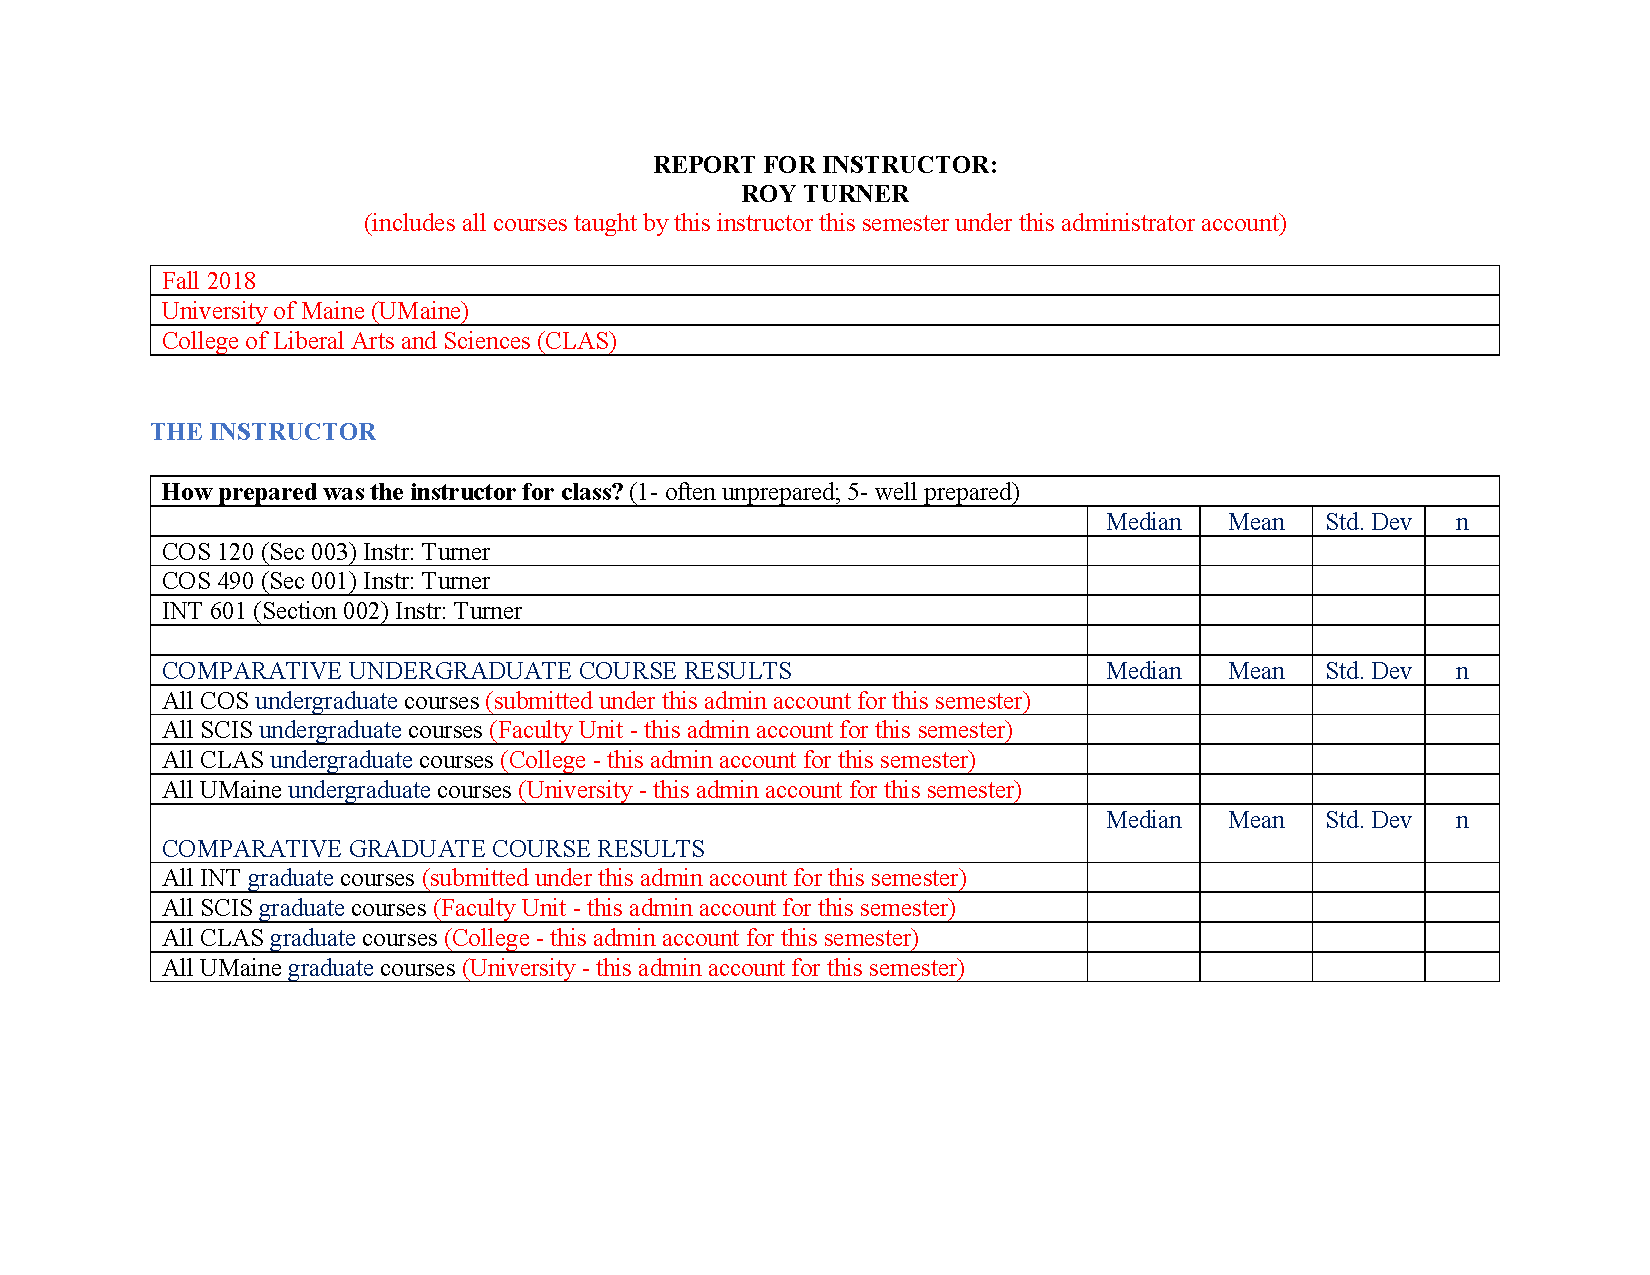
\includepdf[scale=0.85,pages=1,pagecommand=\section{Example Results Display}]{images/results_appendix.pdf}
\includepdf[scale=0.85,pages=2-]{images/results_appendix.pdf}
\end{document}
